\documentclass[a4paper, 14pt]{extarticle}%тип документа

%Русский язык
\usepackage[T2A]{fontenc} %кодировка
\usepackage[utf8]{inputenc} %кодировка исходного кода
\usepackage[english,russian]{babel} %локализация и переносы

%отступы 
\usepackage[left=2cm,right=2cm,top=2cm,bottom=3cm,bindingoffset=0cm]{geometry}

%Вставка картинок
\usepackage{graphicx}
\usepackage{wrapfig, caption}
\graphicspath{}
\DeclareGraphicsExtensions{.pdf,.png,.jpg, .jpeg}
\newcommand\ECaption[1]{%
     \captionsetup{font=footnotesize}%
     \caption{#1}}

%Таблицы
\usepackage[table,xcdraw]{xcolor}
\usepackage{booktabs}

%Графики
\usepackage{pgfplots}
\pgfplotsset{compat=1.9}

%Математика
\usepackage{amsmath, amsfonts, amssymb, amsthm, mathtools}

%Заголовок
\author{Подлесный Артём \\ группа 827}
\title{Работа 1.2.3 \\ Измерение магнитного поля Земли}

\begin{document}
\maketitle
\paragraph*{Цель работы:}определить характеристики шарообразных неодимовых магнитов и, используя
законы взаимодействия магнитных моментов с полем, измерить горизонтальную и вертикальную
составляющие индукции магнитного поля Земли и магнитное наклонение.
\section*{Краткая теория}

Магнитное поле точечного диполя определяется по формуле, аналогичной формуле для поля
элементарного электрического диполя:

\begin{equation}
\vec{B} = \frac{3(\vec{P_m};\vec{r})\vec{r}}{r^5}-\frac{\vec{P_m}}{r^3}.
\end{equation}

В магнитном поле с индукцией $\vec{B}$ на точечный магнитный диполь $\vec{P_m}$ действует механический момент сил:


\begin{equation}
\vec{M} = \vec{P_m} \times \vec{B}.
\end{equation}

В неоднородном поле на точечный магнитный диполь, кроме момента сил, действует ещё и сила:
\begin{equation}
\vec{F} = (\vec{P_m};\vec{\bigtriangledown})\vec{B},
\end{equation}

что в случае сонаправленных магнитных моментов даёт формулу:

\begin{equation}
F = -6\frac{P_m^2}{r^4}.
\end{equation}

Индукция магнитного поля $B_p$ на полюсах однородно намагниченного шара связана с величиной намагниченности $p_m = P_m/V$
и остаточной магнитной индукцией $B_r$
формулой:

\[\vec{B_p} = \frac{2}{3} \vec{B_r} = \frac{8\pi}{3} \vec{p_m} .\]

\section*{Экспериментальное определение величины магнитного момента магнитных шариков (Метод A)}

\begin{wrapfigure}{r}{0.3\textwidth}
\begin{center}
\includegraphics[height=3cm]{teorA.png}
\end{center}
\ECaption{Определение магнитного момента шариков по
силе тяжести (метод A).}
\end{wrapfigure}

Величину магнитного момента $P_m$ одинаковых шариков
можно рассчитать, зная их массу $m$ и определив максимальное расстояние $r_{max}$, на котором они ещё удерживают друг
друга в поле тяжести (см. рис. 1). При максимальном расстоянии сила тяжести шариков равна силе их магнитного притяжения:
\begin{equation}
\dfrac{6P_m^2}{r_{max}^4} = mg \Longrightarrow P_m = \sqrt{\dfrac{mgr_{max}^4}{6}}
\end{equation}

Максимальная величина индукции
наблюдаются на полюсах:

\begin{equation}
\vec{B_p} = \frac{2\vec{P_m}}{R^3}.
\end{equation}

Перед измерением шарики были взвешены на весах, вес используемых шариков был:
\[m = 0.845 \pm 0.005 \text{ г}.\]
Между двумя шариками подкладывалась стопка бумаги, и когда нижний шарик отлипал, получалось искомое расстояние. Учитывая, что диаметр шариков был $d = 6.0 \pm 0.1$ мм, результат:
\[r_{max} = 23.0 \pm 0.1 \text{ мм}.\] 
По полученным данным рассчитываем величину намагниченности по (5):
\[P_m = 62.1 \pm 1.8 \text{ Эрг/Гс},\]
 а так же индукцию на полюсах по формуле (6):
\[B_p = 4603 \pm 287 \text{ Гс}.\]

Так же, с помощью магнетометра АТЕ-8702 поле была измерена индукция на полюсах, которая оказалась равна: 
\[B = 3440 \text{ Гс}.\]
Такое расхождение связано с тем, что скорее всего значение магнетрометра посчитано неверно, так как оно сильно зависит от сканируемой точки, а сам шарик сопоставим по размеру с детектором.

\section*{Определение величины магнитного момента по силе
сцепления магнитных шариков (Метод B)}

\begin{wrapfigure}{l}{0.3\textwidth}
\begin{center}
\includegraphics[height=5cm]{teor.png}
\end{center}
\ECaption{Определение магнитного момента шарика по силе
сцепления (Метод B).}
\end{wrapfigure}

Величину магнитного момента шариков можно
определить также по силе их сцепления. Она определяется как
сила, необходимая для разрыва двух сцепившихся магнитных
шариков. Если сила сцепления двух одинаковых шаров диаметром $d$ c магнитными моментами $P_m$ определяеся (4), то минимальный вес цепочки, при которой она оторвётся от верхнего шарика равен:
\begin{equation}
F = \frac{6P_m^2}{d^4} + \frac{6P_m^2}{(2d)^4} + ... = F_0\left(1+ \frac{1}{2^4}+\frac{1}{3^4}+...\right) \approx 1.08F_0.
\end{equation}

Используя дополнительные шарики, была составлена цепочка из 5 шариков и, с помощью
неодимовых магнитов в форме параллелепипедов, цепочка подсоединена к гирям так, чтобы это был минимальный вес, при котором шарики держались сцепленными. В итогу получившаяся масса, разрывающая шарики, получилась равной:
\[m = 605 \text{ г}.\]
Отсюда по формуле (7) определяем силу магнитов на разрыв:
\[F_0 = 5.5\times 10^5 \text{ Дин}. \]
И, из (4) определяем магнитный момент шарика:
\[P_m = 108.9 \text{ Эрг/Гс}.\]

Это значение сильно больше того, что был померян методом А. Предполагаю, это связано с тем, что цепочка из 5 шариков слишком короткая, чтобы действием сильных неодимовых магнитов можно было пренебречь. Поэтому значение силы разрыва сильно завышено. Скорее всего, значение, померянное методом В - точнее, если бы все измерения были проведены правильно, но в данном случае метод А -точнее, так что в дальнейшем я буду использовать значение, полученное им.

\section*{Измерение горизонтальной составляющей индукции магнитного поля Земли}

\begin{wrapfigure}{l}{0.3\textwidth}
\begin{center}
\includegraphics[height=7cm]{krut.png}
\end{center}
\ECaption{Схема установки крутильного маятника для определения горизонтальной составляющей магнитного поля Земли.}
\end{wrapfigure}


Магнитное поле Земли в настоящей работе определяется по периоду крутильных колебаний
магнитной стрелки вокруг вертикальной оси. 
Магнитная стрелка крутильного маятника показана на рис. 3.
 Магнитные моменты шариков направлены в одну
сторону вдоль оси стрелки. Под действием вращательного
момента $\vec{M} = \vec{P_0} \times\vec{B}$ магнитный момент стрелки $\vec{P_0}$ выстроится вдоль горизонтальной составляющей магнитного поля Земли $\vec{B_h}$ в направлении Юг $\longrightarrow$ Север. 
Даже при 3 шариках, момент инерции $I_n$ такого маятника приблизительно равен моменту инерции однородного стержня. При малых амплитудах $(\sin\theta\approx\theta)$ уравнение колебаний стрелки имеет вид:
\[I_n\ddot{\theta} + P_0B_h\theta=0,\]
отсюда период колебаний маятника из $n$ шариков:
\[T = 2\pi\sqrt{\frac{I_n}{nP_mB_h}}.\]

Таким образом, подставив формулу для момента инерции стрелки, получаем  зависимость периода крутильных колебаний от кол-ва шариков:
\begin{equation}
T(n) = \pi n\sqrt{\frac{md^2}{3P_mB_h}} = kn.
\end{equation}

Перед проведением эксперимента по снятию зависимости $T(n)$ был измерен период крутильных колебаний маятника, обладающего нулевым магнитным моментом. Он получился порядка 25 секунд. Это позволяет перенебречь вкладом натяжения нити в крутильные колебания магнитной стрелки. После этого была снята зависимость для нескольких $n$, изображенная на таблице 1.
\begin{table}[h!]
\begin{center}
\begin{tabular}{|c|c|c|c|c|c|c|c|c|c|}
\hline
\rowcolor[HTML]{9698ED} 
$T_{\text{крут}}$, c & 3.24 & 2.78 & 2.52 & 2.21 & 1.96 & 1.66 & 1.42 & 1.15 & 0.86 \\ \hline
$n$                  & 12   & 10   & 9    & 8    & 7    & 6    & 5    & 4    & 3    \\ \hline
\end{tabular}
\ECaption{Зависимость периода колебаний от количества шариков.}
\end{center}
\end{table}

По этим значениям был построен график, изображенный на рис.4.

\begin{figure}[h!]
\begin{center}
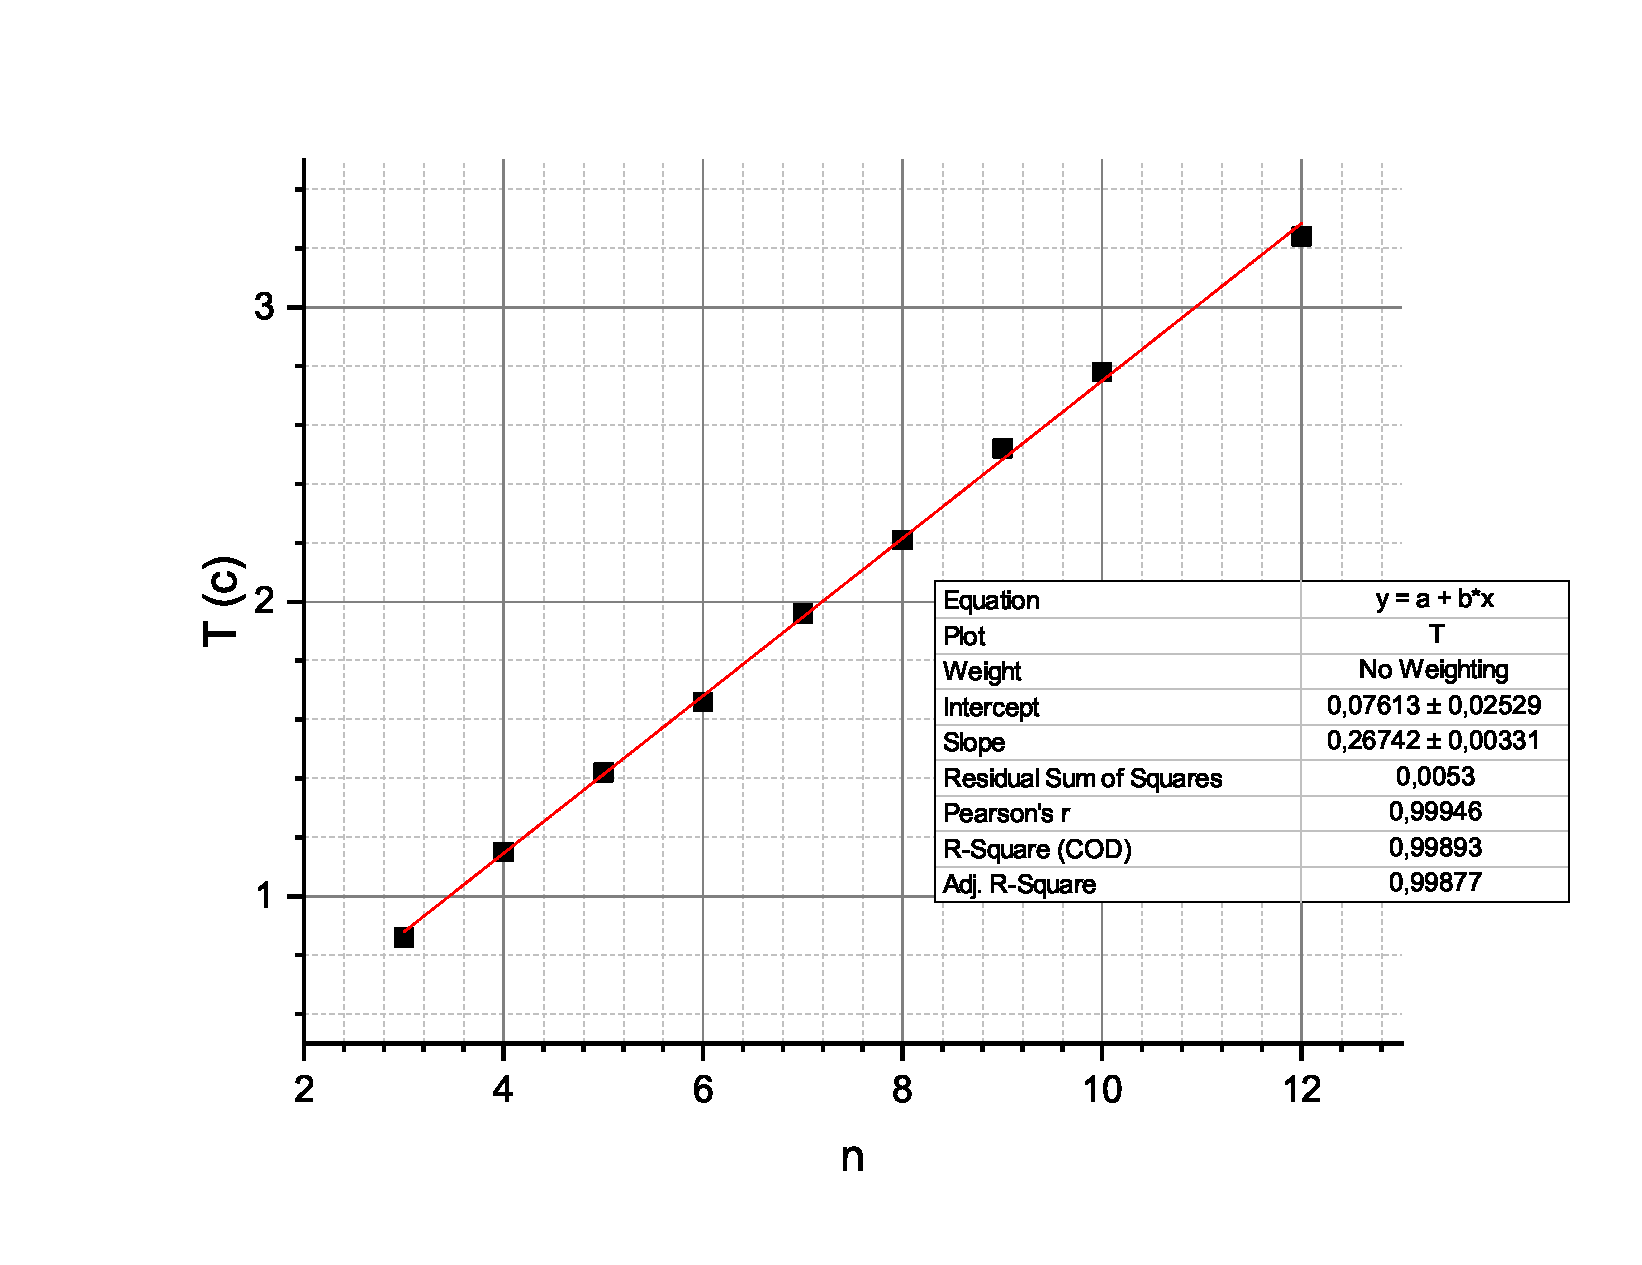
\includegraphics[width=0.9\textwidth]{grkr}
\end{center}
\ECaption{График зависимости $T_{\text{крут}}(n)$. Как видно из графика, он очень хорошо аппроксимируется прямой, что доказывает предположение об аддитивности магнитных моментов шариков, то есть магнитожесткости неодима. }
\end{figure}

Теперь по формуле:
\[B_h = \dfrac{\pi^2md^2}{3k^2P_m},\]
получаем значение для горизонтальной составляющей магнитного поля Земли:
\[B_h = 0.22\pm 0.02 \text{ Гс}.\]
\newpage
\section*{Измерение вертикальной составляющей
индукции магнитного поля Земли.
Магнитное наклонение}

\begin{wrapfigure}{l}{0.5\textwidth}
\begin{center}
\includegraphics[height=7cm]{vert.png}
\end{center}
\ECaption{Схема установки крутильного маятника для определения горизонтальной составляющей магнитного поля Земли.}
\end{wrapfigure}

Для измерения вертикальной $B_v$ составляющей вектора индукции поля Земли используется
та же установка, что и для измерения горизонтальной составляющей с тем лишь отличием,
что магнитная стрелка подвешивается на нити
без $\Lambda$-образного подвеса. В этом случае магнитная стрелка, составленная из чётного числа
шариков и подвешенная на тонкой нити за середину, расположится не горизонтально, а под некоторым, отличным от нуля, углом к горизонту
(см. рис. 4). Это связано с тем, что вектор $\vec{B}$
индукции магнитного поля Земли в общем случае не горизонтален, а образует с горизонтом
угол $\beta$, зависящим от географической широты $\varphi$
места, где проводится опыт. Величина угла $\beta$
называется магнитным наклонением. Можно придать стрелке горизонтальное положение, добавив к одной из сторон грузик известной массы. Тогда момент силы тяжести уравновесит магнитный.
Если масса уравновешивающего
груза равна $m_{\text{гр}}$, плечо силы тяжести $r_{\text{гр}}$, а полный магнитный момент стрелки $P_0 = nP_m$, то
в равновесии: 
\[m_{\text{гр}}gr_{\text{гр}} = nP_mB_v = An.\]

В данном эксперименте была снята зависимость момента силы тяжести от числа шариков $M(n)$, где брались четное кол-во шариков, потому что их удобнее подвешивать за нитку. Эта зависимость представлена на таблице 
2.

\begin{table}[h]
\begin{center}
\begin{tabular}{|c|c|c|c|}
\hline
\rowcolor[HTML]{9698ED} 
$m_{\text{гр}}$, г & $n$ & $r_{\text{гр}}$, см & $M$, эрг     \\ \hline
0.211           & 12  & 3               & 620.34  \\ \hline
\rowcolor[HTML]{9698ED} 
0.209           & 10  & 2.4             & 491.568 \\ \hline
0.233           & 8   & 1.8             & 411.012 \\ \hline
\rowcolor[HTML]{9698ED} 
0.233           & 6   & 1.2             & 274.008 \\ \hline
0.3             & 4   & 0.6             & 176.4   \\ \hline
\end{tabular}
\ECaption{Зависимость момента сил тюжести, уравнивающего магнитный момент вертикальной составляющей магнитного поля Земли, от длины стрелки. }
\end{center}
\end{table}

Теперь по этой зависимости можно построить график, с помощью которого можно определить $B_v$.

\begin{figure}[h!]
\begin{center}
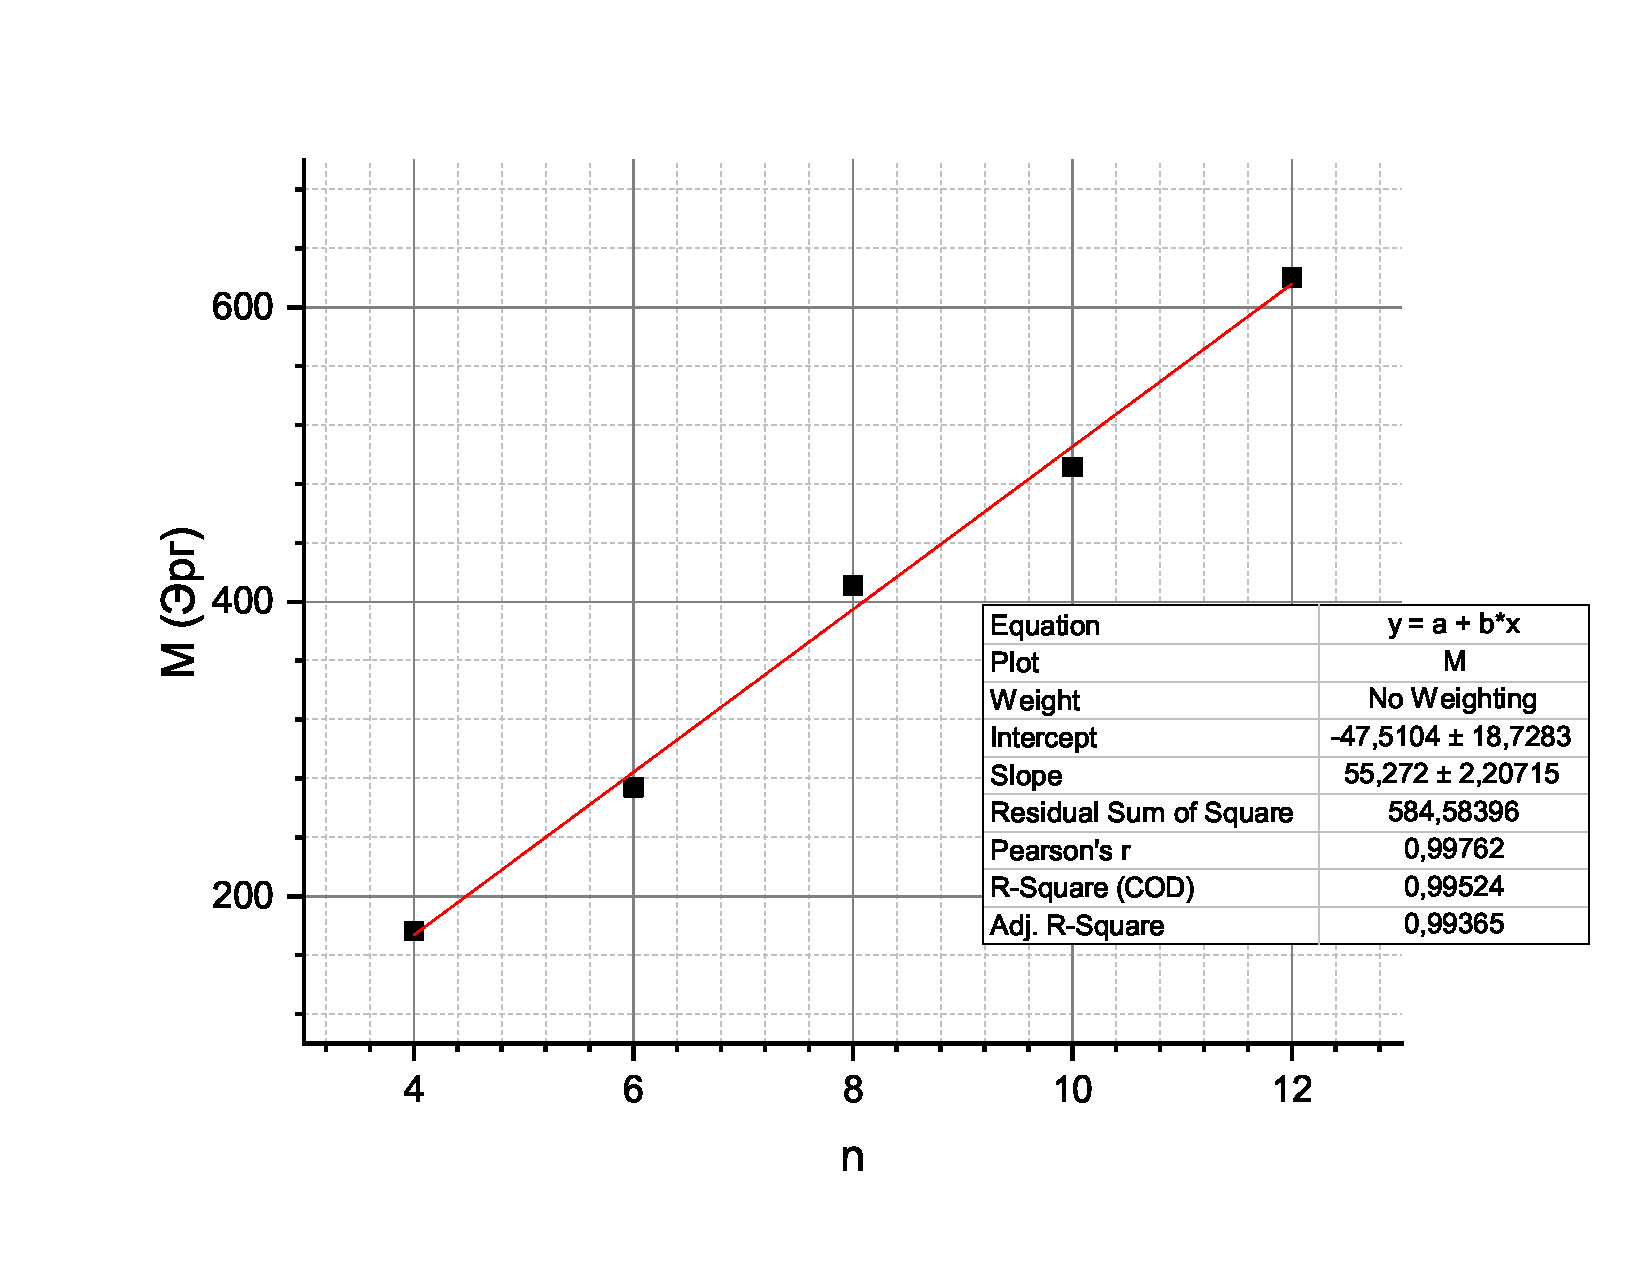
\includegraphics[width=0.9\textwidth]{grvert}
\end{center}
\ECaption{График зависимости $M(n)$. Как видно, он вполне неплохо аппроксимируется прямой, Поэтому можно с малой погрешностью получить значение для  $B_v$. }
\end{figure}

Теперь, зная коэффициент наклона этого графика, можно определить вертикальную составляющую магнитной индукции поля Земли:

\[B_v = \frac{A}{P_m} = 0.88\pm0.06 \text{ Гс}.\]

По полученным результатам, можно найти общую величину магнитного поля $B$ на широте Долгопрудного, а так же величину магнитного наклонения $\beta$:
\[B = \sqrt{B_v^2+B_h^2} = 0.91\pm 0.14\text{ Гс},\]
\[\beta = \arctan\frac{B_v}{B_h} = 76^{\circ}\pm2^{\circ}.\]

Получив эти значения, посчитаем широту, которая теоретически соответствует этому наклонению. Опустив некоторые математические выкладки, получаем следующие теоретические формулы для магнитного поля:
\[B_v = \frac{2p}{r^3}\sin\alpha,\]
где $p$ -- магнитный момент Земли, $r$ -- радиус Земли, $\alpha$  -- широта. Так же:
\[B = \frac{p}{r^3}\sqrt{\frac{5}{2} - \frac{3}{2}\cos2\alpha}.\]
Так как
$\sin\beta = \frac{B_v}{B}$, то окончательно получаем:
\[\alpha = \frac{1}{2}\arcsin\left( \dfrac{2 - \frac{5}{2}\sin^2\beta}{2 - \frac{3}{2}\sin^2\beta}\right)  = 63^{\circ}\pm3^{\circ}.\]

Как видно, результат не совсем сошелся с истинным значением для Долгопрудного: $56^{\circ}$. Однако он неплохо подходит для оценки, так как показал достаточно близкое значение. 
\section*{Вывод}
В работе были измерены магнитные моменты для неодимовых шариков тремя разными методами: уравновешиванием силой тяжести на расстоянии, силой разрыва, а так же магнетрометром. При измерении методом разрыва произошла ошикбка, из-за которой полученное значение получилось слишком завышенным. Магнетроном так же получилось несколько неправильное значение, но этого сложнее избежать из-за малого размера шариков. 

Далее в работе были измерены горизонтальная и вертикальная составлящие магнитного поля Земли, и они дали значение полного поля в Долгопрудном, равное 0.88 Гс, при том, что из справочных данных, магнитное поле Земли колеблется в пределах $0.18\div0.71$ Гс. Я думаю, что основная причина такого отклонения в не совсем правильно посчитанном значении для $P_m$. Скорее всего, из-за того, что бумага по-разному мнется, её толщина была посчитана не совсем правильно в методе А.

Так же было найдено магнитное наклонениие, которое уже теоретически не зависит от величины магнитного момента шарика. На его основании была восстановлена широта Долгопрудного, вполне близкая к реальной. Отклонение скорее всего связано с тем, что шарики были изолированы не ото всех магнитных предметов, что искажало картину поля.






\end{document}